
%(BEGIN_QUESTION)
% Copyright 2015, Tony R. Kuphaldt, released under the Creative Commons Attribution License (v 1.0)
% This means you may do almost anything with this work of mine, so long as you give me proper credit

\noindent
{\bf Lab Exercise -- introduction}

\vskip 5pt

Your task is to build, calibrate, document, and program a flow measurement system consisting of an electronic differential flow transmitter connected to one of the analog inputs of a data acquisition module (DAQ) for a SCADA RTU (Remote Terminal Unit) node which will serve as a {\it flow computer}.  The particular SCADA system we will be using has been designed specifically for BTC Instrumentation students.  It is called {\sl caSCADA} and it is based on a single-board computer running the Linux operating system.  In this lab exercise you will be configuring the RTU node to receive the flow transmitter's analog signal and compute the flow rate of that fluid.  This will involve editing some of the programming code written in the ``C'' language.  Your instructor will assign the flow to be measured, as well as the specific channel(s) to use on the caSCADA system for your loop.

The following table of objectives show what you and your team must complete within the scheduled time for this lab exercise.  Note how some of these objectives are individual, while others are for the team as a whole:

\underbar{Objective completion table:}

% No blank lines allowed between lines of an \halign structure!
% I use comments (%) instead, so that TeX doesn't choke.

$$\vbox{\offinterlineskip
\halign{\strut
\vrule \quad\hfil # \ \hfil & 
\vrule \quad\hfil # \ \hfil & 
\vrule \quad\hfil # \ \hfil & 
\vrule \quad\hfil # \ \hfil & 
\vrule \quad\hfil # \ \hfil & 
\vrule \quad\hfil # \ \hfil & 
\vrule \quad\hfil # \ \hfil \vrule \cr
\noalign{\hrule}
%
% First row
{\bf Performance objective} & {\bf Grading} & {\bf 1} & {\bf 2} & {\bf 3} & {\bf 4} & {\bf Team} \cr
%
\noalign{\hrule}
%
% Another row
Team meeting and prototype sketch (do {\it first!}) & mastery & -- & -- & -- & -- & \cr
%
\noalign{\hrule}
%
% Another row
Circuit design challenge & mastery & & & & & -- -- -- -- \cr
%
\noalign{\hrule}
%
% Another row
Transmitter calibration (with As-Found/As-Left) & mastery & -- & -- & -- & -- &  \cr
%
\noalign{\hrule}
%
% Another row
Spreadsheet characterizing flow element & mastery & -- & -- & -- & -- &  \cr
%
\noalign{\hrule}
%
% Another row
Flow/DP prediction ($\pm$ 5\% of span) & mastery & & & & & -- -- -- -- \cr
%
\noalign{\hrule}
%
% Another row
Linux command-line usage & mastery &  &  &  &  & -- -- -- -- \cr
%
\noalign{\hrule}
%
% Another row
Editing code for transmitter channel & mastery &  &  &  &  & -- -- -- -- \cr
%
\noalign{\hrule}
%
% Another row
Editing code for flow computation channel & mastery & -- & -- & -- & -- &  \cr
%
\noalign{\hrule}
%
% Another row
Final RTU and field wiring inspection & mastery & -- & -- & -- & -- &  \cr
%
\noalign{\hrule}
%
% Another row
%Troubleshooting & mastery &  &  &  &  & -- -- -- -- \cr
%
%\noalign{\hrule}
%
% Another row
Lab question: Instrument connections & proportional &  &  &  &  & -- -- -- -- \cr
%
\noalign{\hrule}
%
% Another row
Lab question: Commissioning & proportional &  &  &  &  & -- -- -- -- \cr
%
\noalign{\hrule}
%
% Another row
Lab question: Math & proportional &  &  &  &  & -- -- -- -- \cr
%
\noalign{\hrule}
%
% Another row
Lab question: Diagnostics & proportional &  &  &  &  & -- -- -- -- \cr
%
\noalign{\hrule}
%
% Another row
Final installation and lab clean-up & mastery & -- & -- & -- & -- &  \cr
%
\noalign{\hrule}
} % End of \halign 
}$$ % End of \vbox

The only ``proportional'' scoring in this activity are the lab questions, which are answered by each student individually.  A listing of potential lab questions are shown at the end of this worksheet question.  The lab questions are intended to guide your labwork as much as they are intended to measure your comprehension, and as such the instructor may ask these questions of your team day by day, rather than all at once (on a single day).

\vskip 10pt

{\bf It is essential that your team plans ahead what to accomplish each day.  A short (10 minute) team meeting at the beginning of each lab session is a good way to do this, reviewing what's already been done, what's left to do, and what assessments you should be ready for.  There is a lot of work involved with building, documenting, and troubleshooting these working instrument systems!}

As you and your team work on this system, you will invariably encounter problems.  You should always attempt to solve these problems as a team before requesting instructor assistance.  If you still require instructor assistance, write your team's color on the lab whiteboard with a brief description of what you need help on.  The instructor will meet with each team in order they appear on the whiteboard to address these problems.





\vfil \eject

\noindent
{\bf Lab Exercise -- team meeting, prototype sketch, and instrument selection}

\vskip 5pt

An important first step in completing this lab project is to {\bf meet with your instructor} as a team to discuss safety concerns, team performance, and specific roles for team members.  If you would like to emphasize exposure to certain equipment (e.g. use a particular type of control system, certain power tools), techniques (e.g. fabrication), or tasks to improve your skill set, this is the time to make requests of your team so that your learning during this project will be maximized.

\vskip 10pt

An absolutely essential step in completing this lab project is to work together as a team to {\bf sketch a prototype diagram} showing what you intend to build.  This usually takes the form of a simple electrical schematic and/or loop diagram showing all electrical connections between components, as well as any tubing or piping for fluids.  This prototype sketch need not be exhaustive in detail, but it does need to show enough detail for the instructor to determine if all components will be correctly connected for their safe function.

For example, if you intend to connect field devices to a PLC (Programmable Logic Controller), your prototype sketch must show how those devices will connect to typical input/output terminals on the PLC, where electrical power will be supplied, etc.  Prototype sketches need not show all intermediary connections between components, such as terminal blocks in junction boxes between the field device and the controller.

You should practice good problem-solving techniques when creating your prototype sketch, such as consulting equipment manuals for information on component functions and marking directions of electric current, voltage polarities, and identifying electrical sources/loads.  Use this task as an opportunity to strengthen your analytical skills!  Remember that you will be challenged in this program to do all of this on your own (during ``capstone'' assessments), so do not make the mistake of relying on your teammates to figure this out for you -- instead, treat this as a problem {\it you} must solve and compare your results with those of your teammates.

Your team's prototype sketch is so important that the instructor will demand you provide this plan before any construction on your team's working system begins.  {\it Any team found constructing their system without a verified plan will be ordered to cease construction and not resume until a prototype plan has been drafted and approved!}  Similarly, you should not deviate from the prototype design without instructor approval, to ensure nothing will be done to harm equipment by way of incorrect connections.  Each member on the team should have ready access to this plan (ideally possessing their own copy of the plan) throughout the construction process.  Prototype design sketching is a skill and a habit you should cultivate in school and take with you in your new career.

\vskip 10pt

In this particular lab, you will most likely use a low-range ``draft'' pressure transmitter to sense the differential pressure created by a primary flow element such as a pitot tube.  DP transmitters designed to sense low pressures in HVAC systems work well for this task if the process fluid is air.  For liquid flow processes, an industrial DP transmitter such as the Rosemount model 3051 should be used instead.  In either case, the transmitter should have a range that can turn down to less than 10 inches water column.

Consult documentation from the manufacturer's website to identify how to properly wire, power, and calibrate the transmitter.  Your instructor will check to see you have located and are familiar with the equipment manual(s).


After locating a suitable instrument and its associated documentation, you should qualitatively test it prior to installing it in your system.  For a pressure transmitter, this entails applying an air pressure to the ``high'' pressure port and measuring the transmitter's milliamp output signal to see if it responds to the application of pressure.  Since the range of this transmitter is so small, the source of air pressure you use must be very low, and could even be your own breath applied to a tube connected to the transmitter's ``H'' port.  If the transmitter fails to respond properly, tag it with a label explaining what it does (or what it fails to do).

\vskip 10pt

{\bf Planning a functioning system should take no more than an hour if the team is working efficiently, and will save you hours of frustration (and possible component destruction!).}






\vfil \eject

\noindent
{\bf Lab Exercise -- building the system}

\vskip 5pt

The major purpose of this lab exercise is to configure the caSCADA system as a {\it flow computer}.  To this end, you may connect any suitable set of transmitters to the caSCADA system for monitoring flow variables, and measure any available fluid flow.  An easy option for flow measurement is {\it wind speed}, treating air as the process fluid and the speed of the wind as the flow to be measured.

\vskip 10pt

The Dwyer corporation sells a ``Mark II'' wind speed indicator, which is essentially a Pitot tube with a vane to constantly maintain its direction pointing upwind.  The differential pressure generated by this self-orienting Pitot tube is conveyed to a differential pressure indicator via a pair of flexible tubes.  In the original Mark II design the DP indicator is a special curved manometer designed to directly indicate wind speed in miles per hour (MPH).  If that manometer is replaced (or supplemented) by an electronic DP transmitter, the analog signal generated may then be input to the data acquisition unit of the caSCADA system and translated into a wind speed indication.

Furthermore, the computational power of the caSCADA system may be put to good use by taking the DP signal sensed from the Mark II Pitot tube and calculating wind speed using a nonlinear formula.  In other words, the DP transmitter may be configured for linear operation, with the RTU computer doing all the necessary calculations to translate this sensed differential pressure into a wind speed.  If multiple DP transmitters are plumbed to the same Pitot tube sensing element, the caSCADA system may be programmed to average those transmitters readings, or perform a selection function on the redundant signals (e.g. low-select, high-select, median-select) to yield a more reliable wind speed measurement.

Alternatively, it is possible to connect temperature, differential pressure, and absolute pressure transmitters to the caSCADA system's analog inputs and have the RTU computer calculate mass flow based on the AGA 3 formula (or something similar to it).

If the flowmeter in question requires no computation for the measurement of flow (e.g. a Coriolis mass flowmeter), then the caSCADA system may be programmed to do some other useful mathematical function, such as recording high and low flow rates, or performing a mass-balance comparison between multiple mass flowmeters in the same system.

\vskip 10pt

Whatever the configuration, the purpose of this system is to showcase the calculation of fluid flow using the computational powers of the caSCADA system, above and beyond a single transmitter registering a single variable.  The wind speed measurement idea is just one possibility, but certainly not the only one acceptable for the purposes of this lab exercise.

\vskip 10pt

The caSCADA RTU nodes are built to operate in outdoor locations, each with its own battery backup power system to continue operation when AC line power fails.  This lends itself to the measurement of real-world flows such as wind speed, water flow in pipes and streams, tidal motion, etc.

Sample diagrams of the caSCADA system wiring, including loop diagram examples, are given in the next question of this worksheet.  The loop diagrams are fairly self-explanatory, and follow a prescribed convention of terminal numbering (versus analog inputs).

%\vskip 10pt

% ADD: images showing various configurations of transmitters connecting to the RTU box for flow computation:
%     --> Three DP identical transmitters on the same flow element, with selector function
%     --> Multiple DP transmitters with different pressure ranges on the same flow element, with large-range selector function
%     --> DP, AP, and T transmitters for mass flow calculation
%     --> Multiple flow transmitters for mass balance calculation in a piping system




\vfil \eject

\noindent
{\bf Lab Exercise -- circuit design challenge}

\vskip 5pt

Your instructor will choose one 4-20 mA field instrument and one control system from the lists shown below, for which you must sketch an accurate circuit diagram showing how the two instruments would connect to each other.  If this interconnection between controller and field instrument requires additional electrical components to function (e.g. DC or AC power source, precision 250 $\Omega$ resistor, diode, relay, etc.), those must be incorporated into your diagram as well.  Instruction manuals for all instrument listed are available on the electronic Instrumentation Reference for your convenience.  When your sketch is complete, you must show the relevant manual pages to your instructor for verification of correct connections.

This exercise tests your ability to locate appropriate information in technical manuals and sketch a correct 4-20 mA loop circuit for a given pair of instruments.  The electronic Instrumentation Reference will be available to you in order to answer this question.

\vskip 10pt

Since all 4-20 mA ``loops'' are basically series DC circuits, it is highly recommended that you approach their design the same as for any other DC circuit: carefully identify all {\it sources} and {\it loads} in the circuit, trace directions of all currents, and mark the polarities of all voltages.  Most of the mistakes made in this type of circuit design challenge may be remedied by careful consideration of these specific circuit-analysis details.


%%%%%%%%%%%%%%%%%%%%%%%%%%%%%%%
\vskip 10pt
\filbreak
\hbox{ \vrule
\vbox{ \hrule \vskip 3pt
\hbox{ \hskip 3pt
\vbox{ \hsize=5in \raggedright

\noindent \centerline{\bf 4-20 mA transmitter options}
\item{} Pressure
\itemitem{} Rosemount 1151 Alphaline (analog), 1151 HART, or 3051 HART
\itemitem{} Yokogawa DPharp EJX110A or EJX910 
\itemitem{} Honeywell ST3000
\vskip 2pt
\item{} Level
\itemitem{} Rosemount APEX non-contact radar, 3300 GWR, or 5300 GWR
\vskip 2pt
\item{} Temperature
\itemitem{} Rosemount 444, 644, 3044, or 3144
\itemitem{} Foxboro RTT15 or RTT30
\itemitem{} Moore Industries SPT with sourcing (4-wire) 4-20 mA output
\itemitem{} Moore Industries SPT with sinking (2-wire) 4-20 mA output
\itemitem{} Moore Industries TRX or TDY
%\itemitem{} Honeywell STT173
\vskip 2pt
\item{} Flow
\itemitem{} Foxboro CFT50 coriolis
\vskip 2pt
\item{} Analytical
\itemitem{} Rosemount 5081-P (pH)
\itemitem{} Daniel 700 gas chromatograph (4 analog output channels)
\itemitem{} Foxboro 876PH (pH/ORP/ISE)
\end{itemize}

} \hskip 3pt}%
\vskip 5pt \hrule}%
\vrule}
%%%%%%%%%%%%%%%%%%%%%%%%%%%%%%%




%%%%%%%%%%%%%%%%%%%%%%%%%%%%%%%
\vskip 10pt
\filbreak
\hbox{ \vrule
\vbox{ \hrule \vskip 3pt
\hbox{ \hskip 3pt
\vbox{ \hsize=5in \raggedright

\noindent \centerline{\bf Controller options}
\item{} Monolithic
\itemitem{} Siemens 352P 
\itemitem{} Siemens 353
\itemitem{} Foxboro 716C
\itemitem{} Foxboro 718TC
\itemitem{} Foxboro 762CNA 
\itemitem{} Moore Industries 535
\itemitem{} Honeywell UDC2300
\itemitem{} Honeywell UDC3500 
\vskip 2pt
\item{} Modular -- {\it you choose the appropriate I/O module}
\itemitem{} Siemens 353R 
\itemitem{} Emerson ROC800 SCADA/RTU 
\vskip 2pt
\item{} Distributed Control System (DCS) -- {\it you choose the appropriate I/O module}
\itemitem{} Emerson DeltaV with M-series I/O
\itemitem{} Emerson DeltaV with S-series I/O 
\itemitem{} Honeywell Experion with 2MLF series I/O 
\vskip 2pt
\item{} Programmable Logic Controller (PLC) -- {\it you choose the appropriate I/O module}
\itemitem{} Siemens S7-300 
\itemitem{} Rockwell ControlLogix (catalog number 1756)
\itemitem{} Rockwell CompactLogix (catalog number 1769)
\end{itemize}

} \hskip 3pt}%
\vskip 5pt \hrule}%
\vrule}
%%%%%%%%%%%%%%%%%%%%%%%%%%%%%%%




%%%%%%%%%%%%%%%%%%%%%%%%%%%%%%%
\vskip 10pt
\filbreak
\hbox{ \vrule
\vbox{ \hrule \vskip 3pt
\hbox{ \hskip 3pt
\vbox{ \hsize=5in \raggedright

\noindent \centerline{\bf 4-20 mA Final Control Element options}
\item{} Pneumatic control valve positioners
\itemitem{} Fisher 3582i positioner 
\itemitem{} Fisher DVC6000 positioner 
\vskip 2pt
\item{} Electrically actuated valves (MOV)
\itemitem{} Limitorque actuator with Modutronic-20 II controller 
\itemitem{} Rotork AQ with Folomatic controller 
\vskip 2pt
\item{} AC motor drives (VFD)
\itemitem{} Rockwell PowerFlex 4 
\itemitem{} Automation Direct GS1 
\end{itemize}

} \hskip 3pt}%
\vskip 5pt \hrule}%
\vrule}
%%%%%%%%%%%%%%%%%%%%%%%%%%%%%%%


\vfil

Study reference: the ``Analog Electronic Instrumentation'' chapter of {\it Lessons In Industrial Instrumentation}, particularly the section on HART.

\vskip 10pt

Note: a very effective problem-solving strategy for determining how to connect different components together to create a working 4-20 mA current loop is to first identify whether each component acts as a {\it source} or a {\it load} in that loop circuit.  Then, label voltage polarities (+ , $-$) and directions of current accordingly.  Knowing which way current must flow through each component and which polarity each voltage must have is key to ensuring the inter-component connections are correct.







\vfil \eject

\noindent
{\bf Lab Exercise -- instrument calibration}

\vskip 5pt

If your team's flow transmitter is based on pressure, you must calibrate the differential pressure transmitter (``trim'' both the sensor and the output) to ensure it interprets pressure accurately and outputs an accurate current.

As in all cases where an instrument must be calibrated, you will need to check the instrument's response against one or more {\it standards}.  In this case, the ideal standard to use for setting the input pressure to the transmitter is a {\it manometer}, and the ideal standard to use for measuring the transmitter's electronic output signal is a {\it multimeter} configured to measure DC milliamps:

$$\includegraphics[width=15.5cm]{i02865x02.eps}$$

It is entirely permissible for teams to share one transmitter.  No matter how well-calibrated one team might have left a transmitter, there is always room for another team to re-calibrate that same transmitter and at least attempt to calibrate it better.  A comparison of your team's As-Found versus As-Left values will demonstrate the improvement(s) you were able to make.

\vskip 10pt

It should be noted that when calibrating pressure transmitters with very low ranges, as is often the case when measuring flow in a lab environment, the physical mounting position of the transmitter may make a significant difference in its calibration.  If the transmitter is re-oriented, gravity will tug at the pressure-sensing element in a different direction and thereby cause its calibration to shift.  This shift is typically just a ``zero'' error, and is therefore fairly easy to correct, but it will necessitate another calibration check in the field.  A good field test, therefore, is to mount the transmitter in its final position and then check its analog output signal with zero differential pressure applied (i.e. with the equalizing valve of a three-valve manifold opened, or by connecting the ``H'' and ``L'' ports of the transmitter together with a tube to absolutely ensure no differential pressure exists.

\filbreak

Document the accuracy of your transmitter's sensor trim before and after adjustment in this table, at five different points throughout its sensing range using these two tables:

\vskip 10pt

{\bf As-Found calibration table}

% No blank lines allowed between lines of an \halign structure!
% I use comments (%) instead, so that TeX doesn't choke.

$$\vbox{\offinterlineskip
\halign{\strut
\vrule \quad\hfil # \ \hfil & 
\vrule \quad\hfil # \ \hfil & 
\vrule \quad\hfil # \ \hfil & 
\vrule \quad\hfil # \ \hfil \vrule \cr
\noalign{\hrule}
%
% First row
Applied pressure & Output signal (actual) & Output signal (ideal) & Error (\% of span) \cr
%
\noalign{\hrule}
%
% Another row
 &  &  & \cr
%
\noalign{\hrule}
%
% Another row
 &  &  & \cr
%
\noalign{\hrule}
%
% Another row
 &  &  & \cr
%
\noalign{\hrule}
%
% Another row
 &  &  & \cr
%
\noalign{\hrule}
%
% Another row
 &  &  & \cr
%
\noalign{\hrule}
} % End of \halign 
}$$ % End of \vbox

\vskip 10pt

{\bf As-Left calibration table}

% No blank lines allowed between lines of an \halign structure!
% I use comments (%) instead, so that TeX doesn't choke.

$$\vbox{\offinterlineskip
\halign{\strut
\vrule \quad\hfil # \ \hfil & 
\vrule \quad\hfil # \ \hfil & 
\vrule \quad\hfil # \ \hfil & 
\vrule \quad\hfil # \ \hfil \vrule \cr
\noalign{\hrule}
%
% First row
Applied pressure & Output signal (actual) & Output signal (ideal) & Error (\% of span) \cr
%
\noalign{\hrule}
%
% Another row
 &  &  & \cr
%
\noalign{\hrule}
%
% Another row
 &  &  & \cr
%
\noalign{\hrule}
%
% Another row
 &  &  & \cr
%
\noalign{\hrule}
%
% Another row
 &  &  & \cr
%
\noalign{\hrule}
%
% Another row
 &  &  & \cr
%
\noalign{\hrule}
} % End of \halign 
}$$ % End of \vbox

When finished calibrating your team's transmitter, be sure to place a calibration tag on it showing the range and the date it was calibrated.  A set of calibration tags are shown here which you may cut out and tape to the transmitter after completing your calibration:

$$\includegraphics[width=15.5cm]{i02865x01.eps}$$

If your team's flow transmitter is not pressure-based (e.g. vortex, magnetic, turbine, Coriolis, etc.) then the input standard you must provide for calibration will not be pressure.  In some cases the input standard may be electrically simulated (e.g. simulating the voltage induced by the flowtube in a magnetic flowmeter), but in other cases you may have to do a ``bucket test'' which involves timing how long it takes to fill a bucket of known volume with the liquid passing through the flowmeter.

\vskip 10pt

{\bf Common mistakes:}

\begin{itemize}
\item{} Choosing a calibration (``trim'') range that is substantially less than the final range of measurement when installed.  As a general rule, you should trim the sensor of the transmitter to cover the broadest range of measurement possible with your calibration equipment.
\item{} Changing the physical orientation of the differential pressure transmitter between calibration and field mounting, without re-trimming the sensor's zero point.  
\item{} Neglecting to place a calibration tag on the transmitter after calibrating it.
\end{itemize}

\vskip 10pt

{\bf Characterizing your team's flow element and calibrating your team's transmitter to match should take no more than one full lab session (3 hours) if the team is working efficiently!}






\vfil \eject

\noindent
{\bf Lab Exercise -- flow element characterization}

\vskip 5pt

Flowmeters based on the generation of a differential pressure (DP) by acceleration or deceleration of the fluid are inherently non-linear in nature: doubling the flow rate results in approximately quadrupling the DP generated.  In order to be able to program the caSCADA system to accurately compute flow rate from differential pressure measurements, you must {\it characterize} the flow element.  This means testing the flow element against known flow rates to see how much pressure it generates at those rates, and then deriving a formula relating pressure to flow rate.  You may think of this as analogous to developing a {\it strapping table} for tank liquid level measurement: exposing the sensor to a set of known values to see how it responds across a wide range of values, and then recording those values for later use in interpreting the process variable.

An important tool for this task is an {\it electronic spreadsheet program} such as Microsoft Excel.  You will take the flow/DP data measured for your flow element, enter those data points in a spreadsheet, and have the spreadsheet plot a graph of the data with DP as the independent variable (horizontal axis) and flow rate as the dependent variable (vertical axis).  Most spreadsheets permit both linear and logarithmic plotting, which should generate a pair of plots looking something like this:

$$\includegraphics[width=15.5cm]{i02865x03.eps}$$

Flow elements such as orifice plates, venturi tubes, Pitot tubes, and flow nozzles should exhibit a simple quadratic characteristic, represented by the formula $Q = k \sqrt{\Delta P}$.  Logarithmic scales are very helpful when graphing inherently nonlinear functions such as this.  Note what happens to this quadratic function when the logarithm is taken of both sides:

$$Q = \sqrt{\Delta P} = \Delta P^{1/2}$$

$$\log Q = \log \Delta P^{1/2}$$

$$\log Q = {1 \over 2} \log \Delta P$$

$${{\log Q} \over {\log \Delta P}} = {1 \over 2}$$

Thus, a graph of the {\it logarithm} of $Q$ plotted with respect to the {\it logarithm} of $\Delta P$ yields a line with constant slope of one-half ($1 \over 2$).  Deviations from the ideal quadratic function are more readily seen in such a log/log plot because they appear as deviations from a straight line.  It is more difficult for a person to detect the same deviations on a graph when the ideal plot is a curve instead of a line.

\vskip 10pt

\filbreak

Another powerful feature of electronic spreadsheets is their ability to {\it fit a mathematical function} to your data.  Once you have plots of your flow/DP data, you will instruct the spreadsheet to trace a function over that same data to mathematically approximate it.  In Microsoft Excel, this feature is called a {\it trendline}, which may be enabled and configured by right-clicking on any of the points on the plotted function.  This function in the form of $y = f(x)$ will be something you may then program into the caSCADA system to convert $x$ (differential pressure) into $y$ (flow rate or flow velocity).  The formula fit by the spreadsheet will likely be more accurate to your flow element than $Q = k \sqrt{\Delta P}$ because the latter is based on theory while the former is based on empirical data from your flow element.

\vskip 10pt

This is the end-goal of your spreadsheet use in this lab exercise: to generate a formula relating differential pressure (in inches water column) to flow rate (e.g. volumetric units, or mass units, or flowing velocity).  Your team must show your spreadsheet to the instructor, explain how you plotted the data and displayed the trendline formula, and explain what the data and formula mean.

\vskip 10pt

{\bf Common mistakes:}

\begin{itemize}
\item{} Not recording enough data points.  There really is no maximum number of data points to collect during your characterization test.  The more data points, the better, because it means the spreadsheet will have more data to analyze in deriving its mathematical function, and that function will likely be a better fit to the true measurement!
\item{} Not recognizing poor data.  The data you collect during the characterization process should closely resemble the function predicted by theory.  If you see one or more data points that deviate substantially from the smooth curve connecting the other data points together (i.e. ``outliers''), something likely went wrong during the testing process and it should be repeated.
\item{} Reversing the axes on the plots.  Remember, in order for the spreadsheet-generated formula to be useful to you in programming the caSCADA system, differential pressure must be the independent variable ($x$) and flow must be the dependent variable ($y$).
\end{itemize}









\vfil \eject

\noindent
{\bf Lab Exercise -- flow/DP prediction}

\vskip 5pt

Regardless of the type of flowmeter used by your team to measure process flow rate, everyone must also demonstrate competence calculating differential pressure generated by a DP-based flow element given a known flow rate, or vice-versa.  A system called the {\it turbocompressor} already exists in the main lab room with a variable-frequency-driven air fan blowing air through a venturi tube, and an indicating differential pressure transmitter sensing the DP generated by that venturi tube.  Air flow rate is a direct (linear) function of the fan's speed, which is a direct (linear) function of the motor's drive frequency.

\vskip 10pt

The mathematical relationship between flow rate and DP for any given flow element and fluid type, of course, is given by the following formula:

$$Q = k \sqrt{\Delta P}$$

\noindent
Where,

$Q$ = Flow rate

$k$ = Proportionality constant

$\Delta P$ = Differential pressure

\vskip 10pt

The ``k factor'' of this venturi tube assembly may be derived by manipulating that formula to solve for $k$ and plugging in known values of $Q$ (i.e. fan drive frequency) and $\Delta P$.  Known values for one particular fan speed will be provided by the instructor prior to each student's challenge.  After providing these $Q$ and $\Delta P$ values, the instructor will then randomly change the fan's speed and either hide that new fan speed or hide the new $\Delta P$ value, and have each student calculate the hidden value based on the {\it other} value which will be evident for all to see.

\vskip 10pt

Each student passes this challenge when they are able to correctly calculate the hidden variable from the revealed variable.









\vfil \eject

\noindent
{\bf Linux command-line usage}

\vskip 5pt

The caSCADA telemetry system is built on the foundation of a single-board computer called a ``Raspberry Pi'' running the Linux operating system.  Linux is a free and open-source version of the venerable Unix operating system which was developed for large mainframe computers in the early 1970's.  In this lab exercise you will demonstrate competence using additional typed commands for the Linux operating system, in addition to using the commands you have already learned.

\vskip 20pt

%\vfil \eject

\vbox{\hrule \hbox{\strut \vrule{} {\tt man} \vrule} \hrule} 

A standard feature of all Unix systems is the {\it manual} library with documentation on virtually all commands and installed software.  This documentation is available at the command line simply by typing {\tt man} followed by the name of the command or program you wish to learn about.  For example, if you wished to learn how to properly use the {\tt ifconfig} command to view network parameters, you would type {\tt man ifconfig}.  The screen then switches to a display of the ``manual'' page for that command, where you may scroll up and down using arrow keys and page up/down keys, and search for terms by pressing the {\tt /} key.  You may exit the manual page at any time by pressing the {\tt q} key.





\vskip 20pt

%\vfil \eject

\vbox{\hrule \hbox{\strut \vrule{} {\tt cp} \vrule} \hrule} 

The {\tt cp} command makes a {\it copy} of a file.  Both the original file name and the new (copied) file name are specified, in that order, as arguments to the {\tt cp} command.  For example, entering the command {\tt cp data.txt mydata} copies the contents of the text file {\tt data.txt} into a new file within that same directory named {\tt mydata}.

You can get creative with directories using the {\tt cp} command, too.  For example, the command {\tt cp caSCADA/cascada.h ../header.h} copies the contents of the file {\tt cascada.h} located in the subdirectory {\tt caSCADA} into a new file named {\tt header.h} residing one directory level above ({\tt ../}) where we are currently navigated.  If we were to omit the ``header.h'' from the last argument it would copy the {\tt cascada.h} file to the new location but as its original file name.

Without any options specified, the {\tt cp} command acts silently, not prompting for confirmation of a file's duplication or even giving any indication that the job is done.  For this reason, I prefer to get into the habit of including the {\tt v} (``verbose'') and {\tt i} (``interactive'') options when invoking the {\tt cp} command.  If you were to type {\tt cp -vi data.txt mydata} and press Enter, it would prompt you with a question to confirm whether you really wanted to copy this file if indeed a file named {\tt mydata} already existed (press {\tt y} to confirm and {\tt n} to escape) which is the ``interactive'' option at work.  It would also tell you the file had been copied when complete -- that's the ``verbose'' option at work.




\vskip 20pt

%\vfil \eject

\vbox{\hrule \hbox{\strut \vrule{} {\tt mv} \vrule} \hrule} 

The {\tt mv} command does the same thing as the {\tt cp} command, but deletes the original file after the copying process is complete.  In other words, the {\tt mv} command {\it moves} the file rather than duplicating it.  Like the {\tt cp} command, the {\tt mv} command also obeys the {\tt -vi} options.  This is highly recommended as a habit to build, as it will save you someday from accidently relocating a file.



%\vskip 20pt

\vfil \eject

\vbox{\hrule \hbox{\strut \vrule{} {\tt rm} \vrule} \hrule} 

Okay, here is where we could potentially do some permanent damage to the system!  The {\tt rm} command removes, or deletes, any file specified.  If you were to type {\tt rm data.txt} it would delete any file named {\tt data.txt}.  Like the copy ({\tt cp}) command, {\tt rm} supports both the ``verbose'' and ``interactive'' options which are highly recommended to avoid accidental deletions.

To get some practice using this command, you will need to have some files available that are safe to delete.  Two such files are the {\tt data.txt} and {\tt data.html} files which are refreshed and re-written periodically any time the {\tt poll} or {\tt simulate} caSCADA processes are running.  Another way to practice using the {\tt rm} command is to first use the {\tt touch} command to create a new file of zero byte size which you may then delete (e.g. typing {\tt touch junk} creates a new file named ``junk'' which of course is safe for anyone to remove).





\vskip 20pt

%\vfil \eject

\vbox{\hrule \hbox{\strut \vrule{} {\tt *} \vrule} \hrule} 

The asterisk symbol isn't really a command, but rather a ``wildcard'' character useful for representing portions of file names or directory names.  Specifically, the asterisk character represents {\it any} one or multiple characters that might be part of a file name or directory name.  For example, if you were to issue the command {\tt ls -l *.txt} it would display a listing of all files ending with the {\tt .txt} extension (i.e. all text files). 

The asterisk wildcard may be used at the beginning, middle, or even end of a specified file or directory name.  Note the following examples:

\vskip 10pt

{\tt cd engineer*} \hskip 20pt {\it Relocates you to the directory beginning with the letters ``engineer''.  If more than one directory is so named, this will return an error message.}

\vskip 10pt

{\tt rm -vi junk*txt} \hskip 20pt {\it Removes all files having names beginning with the letters ``junk'' and ending with the letters ``txt''.}

\vskip 10pt

{\tt cp -vi *poll* ../../} \hskip 20pt {\it Copies all files containing the letters ``poll'' in their names two directory levels above where we are right now.  If multiple files exist fitting this name pattern, all of them will be copied to that location under their original names.}

\vskip 10pt

Another wildcard character that is sometimes useful is the {\tt ?} which is a wildcard {\it only for a single character} in a file name or directory name, versus {\tt *} which is a wildcard for any number of consecutive characters in a name.




\vskip 20pt

%\vfil \eject

\vbox{\hrule \hbox{\strut \vrule{} {\tt mkdir} \vrule} \hrule} 

This command creates (``makes'') a new subdirectory under the directory you happen to presently reside.  The name of the new subdirectory must be specified as an argument to the {\tt mkdir} command.  For example, if you were to type {\tt mkdir Elvis} it would create a new subdirectory named {\tt Elvis}.




\vskip 20pt

%\vfil \eject

\vbox{\hrule \hbox{\strut \vrule{} {\tt rmdir} \vrule} \hrule} 

This command deletes (``removes'') a specified subdirectory.  For example, {\tt rmdir Elvis} will delete the {\tt Elvis} subdirectory, but only if that directory is empty.  The {\tt rmdir} command does nothing if there are files located within the specified subdirectory, acting out of precaution.



\vfil \eject

\vbox{\hrule \hbox{\strut \vrule{} {\tt grep} \vrule} \hrule} 

This highly useful command scans a text file and prints to the screen only those lines within the file containing a specified string of text you specify as an argument to the command.  For example, if you were to type the command {\tt grep PT-45 data.txt} it would scan the file {\tt data.txt} and only print out those lines of the file containing the text {\tt PT-45}.  The text string {\tt grep} searches for is case-sensitive, and must be spelled perfectly.  If space characters are part of the desired search string, you will need to enclose the text string in quotation marks (e.g. {\tt grep "Is anyone there" letter.txt}) in order to not interpret the space characters between {\tt Is} and {\tt anyone} and {\tt there} as delimiters between additional arguments to the {\tt grep} command.  If we were to have omitted the quotation marks, {\tt grep} would only have searched for the text string {\tt Is}, but it would have looked for that string within three different files: {\tt anyone}, {\tt there}, and {\tt letter.txt}!

As you can probably guess, the {\tt grep} command is very useful when using the caSCADA system, as it allows you to scan any of the live data files updated by the {\tt poll} or {\tt simulate} processes for just the channel you are interested in.


\vskip 20pt

%\vfil \eject

\vbox{\hrule \hbox{\strut \vrule{} {\tt grep -v} \vrule} \hrule} 

The {\tt -v} option for the {\tt grep} command instructs it to obey an {\it inverse match} rule.  That is to say, the {\tt -v} option tells {\tt grep} to search for lines in a file that {\it do not} contain the text string you specify.



\vskip 20pt

%\vfil \eject

\vbox{\hrule \hbox{\strut \vrule{} {\tt |} \vrule} \hrule} 

Like the asterisk character ({\tt *}), the ``pipe'' character ({\tt |}, which is located on most keyboards as the shift-character on the backslash key) isn't really a command at all, but rather a different kind of function in the Unix command-line environment.  The ``pipe'' character links two or more commands together, so that the text output of the first command gets sent as input into the next command, as though those two commands were linked together with a section of virtual pipe.

One of the most common uses of such ``plumbing'' in Unix systems is the pipe a command to the {\tt grep} command to filter for a particular string of text.  Consider, for example, the {\tt ps -e} command, which displays to the terminal a list of all ``processes'' currently running on the computer.  If you wished to scan that list of running processes to look for a particular process name, or process ID number, or terminal ID, it could be very tedious and error-prone to do it manually by visually scanning the list with your eyes.  Instead, we could issue the {\tt ps -e} command followed by the pipe symbol and then use {\tt grep} to display only certain lines.  For example, the command {\tt ps -e | grep poll} will display all instances of processes running which contain the string ``poll'' anywhere in the line output by {\tt ps}.









\vfil \eject

\noindent
{\bf Editing and running caSCADA code}

\vskip 5pt

For each transmitter connected to the DAQ unit in the RTU, there will be one designated caSCADA channel.  For a flow measurement system with three redundant pressure transmitters sensing DP generated by a common flow element, this means three channels: one for each of the redundant transmitters.  

Each of these transmitter channels will be scaled linearly, representing the variable directly sensed by the transmitter.  If the transmitters in question sense differential pressure, then the scaled value will be in units appropriate to differential pressure rather than units appropriate to flow.  A new requirement for this lab exercise is that the transmitter channel must employ conditional (``if'') statements to set the channel's status value to something other than 1 if the reading falls outside of the proper or usable range.

Additional channel(s) will be designated on the caSCADA system for the computation of flow rate.  These channels will take value and status data from the transmitter channels and perform appropriate mathematical calculations on that data to convert it into a flow rate.  It is each {\it team's} responsibility to edit the C code for a flow-computation channel.

\vskip 10pt

For example, suppose the system you're assigned will have three redundant DP transmitters wired to analog inputs 1, 2, and 3 on the LabJack DAQ.  Each of the channel functions will be written to scale the 4-20 mA signal into appropriate pressure readings, as shown in this example code for the file {\tt f\_channel\_02.c} which takes in the 1-5 VDC analog signal and scales it into 0-5 inches WC differential pressure.  Here, the status is set to 0 if the transmitter becomes under-ranged (less than 0.0) or over-ranged (more than 5.0):

\vskip 10pt

\hbox{ \vrule
\vbox{ \hrule \vskip 3pt
\hbox{ \hskip 3pt
\vbox{ \hsize=6in \raggedright

{\tt /**********************************************************}

{\tt Consult the "README.txt" file for help editing this function!}

{\tt **********************************************************/}

\vskip 10pt

{\tt \#include <stdio.h>}

{\tt \#include <math.h>	    // Necessary for any advanced math functions}

{\tt \#include "cascada.h"  // Contains all the declarations specific to caSCADA}

\vskip 10pt

{\tt int}

{\tt f\_channel\_02 (void)}

$\lbrace$

\vskip 10pt

\hskip 10pt {\tt  f\_channel[2].value = ain[2] * 1.25 - 1.25;}

\hskip 10pt {\tt  f\_channel[2].tag = "PDT-102";}

\hskip 10pt {\tt  f\_channel[2].unit = "Inches WC";}

\vskip 10pt

\hskip 10pt {\tt  if (f\_channel[2].value < 0.0 || f\_channel[2].value > 5.0)}

\hskip 20pt {\tt  f\_channel[2].status = 0;}

\vskip 10pt

\hskip 10pt {\tt  else}

\hskip 20pt {\tt  f\_channel[2].status = 1;}

\vskip 10pt

\hskip 10pt {\tt  f\_channel[2].comment = "Redundant DP transmitter number 2";}

\vskip 10pt

\hskip 10pt {\tt return 1;}

$\rbrace$

}
\hskip 3pt}%
\vskip 5pt \hrule}%
\vrule}

\vskip 10pt

Since each student will be responsible for editing the transmitter channel code, the instructor will assign different ``if'' conditions to every student to ensure a genuine learning experience.  For example, the instructor may assign a different threshold for a ``bad'' (0) status value on a DP transmitter: perhaps any signal less than 10\% of the scaled range rather than only for values less than zero.  Alternatively, the instructor may request that the comment change dynamically with the status as well.

\vfil \eject

Using conditional (``if'') expressions in C language programming is a new objective and requires new knowledge.  First, a list of the relational (comparative) and logical (AND/OR) operators used by the {\tt if} conditional:

% No blank lines allowed between lines of an \halign structure!
% I use comments (%) instead, so that TeX doesn't choke.

$$\vbox{\offinterlineskip
\halign{\strut
\vrule \quad\hfil # \ \hfil & 
\vrule \quad\hfil # \ \hfil \vrule \cr
\noalign{\hrule}
%
% First row
{\bf Relational operator} & {\bf Meaning} \cr
%
\noalign{\hrule}
%
% Another row
== & Equal to \cr
%
\noalign{\hrule}
%
% Another row
!= & Not equal to \cr
%
\noalign{\hrule}
%
% Another row
$<$ & Less than \cr
%
\noalign{\hrule}
%
% Another row
$<=$ & Less than or equal to \cr
%
\noalign{\hrule}
%
% Another row
$>$ & Greater than \cr
%
\noalign{\hrule}
%
% Another row
$>=$ & Greater than or equal to \cr
%
\noalign{\hrule}
} % End of \halign 
}$$ % End of \vbox


% No blank lines allowed between lines of an \halign structure!
% I use comments (%) instead, so that TeX doesn't choke.

$$\vbox{\offinterlineskip
\halign{\strut
\vrule \quad\hfil # \ \hfil & 
\vrule \quad\hfil # \ \hfil \vrule \cr
\noalign{\hrule}
%
% First row
{\bf Logical operator} & {\bf Meaning} \cr
%
\noalign{\hrule}
%
% Another row
{\tt \&\&} & AND \cr
%
\noalign{\hrule}
%
% Another row
{\tt ||} & OR \cr
%
\noalign{\hrule}
} % End of \halign 
}$$ % End of \vbox

Next, some examples of {\tt if} conditionals shown in code snippets (with explanatory comments).  This first example sets the status to different values depending on if the measurement is under-ranged, over-ranged, or within range:

\vskip 10pt

\hbox{ \vrule
\vbox{ \hrule \vskip 3pt
\hbox{ \hskip 3pt
\vbox{ \hsize=6in \raggedright

%$\lbrace$

\hskip 10pt {\tt  if (f\_channel[2].value < 0.0)}

\hskip 20pt {\tt  f\_channel[2].status = 0;  \hskip 50pt  // Sets status = 0 if negative}

\vskip 10pt

\hskip 10pt {\tt  else if (f\_channel[2].value > 5.0)}

\hskip 20pt {\tt  f\_channel[2].status = 2;  \hskip 50pt  // Sets status = 2 if over 5.0 inches WC}

\vskip 10pt

\hskip 10pt {\tt  else}

\hskip 20pt {\tt  f\_channel[2].status = 1;  \hskip 50pt  // Sets status = 1 if neither}

%$\rbrace$

}
\hskip 3pt}%
\vskip 5pt \hrule}%
\vrule}

\vskip 10pt

Pay close attention to which lines are terminated with semicolon characters ({\tt ;}) and which are not.  Every ``action'' statement ends with one, but the {\tt if} conditional lines do not.

\vskip 20pt

This next example takes multiple actions with each condition of the measurement.  Note the use of curly-brace characters to encompass all the statements executed for a given condition, which were not needed when there was only one statement executed per ``if'' condition:

\vskip 10pt

\hbox{ \vrule
\vbox{ \hrule \vskip 3pt
\hbox{ \hskip 3pt
\vbox{ \hsize=6in \raggedright

\hskip 10pt {\tt  if (f\_channel[2].value < 0.0 || f\_channel[2].value > 5.0)}

\hskip 10pt $\lbrace$

\hskip 20pt {\tt  f\_channel[2].status = 0;  \hskip 80pt  // Sets status = 0 if out of range}

\hskip 20pt {\tt  f\_channel[2].comment = "Out of range";  \hskip 10pt  // Sets comment too}

\hskip 10pt $\rbrace$

\vskip 10pt

\hskip 10pt {\tt  else}

\hskip 10pt $\lbrace$

\hskip 20pt {\tt  f\_channel[2].status = 1;  \hskip 80pt  // Sets status = 1 if range is good}

\hskip 20pt {\tt  f\_channel[2].comment = "Range okay";  \hskip 18pt  // Sets comment too}

\hskip 10pt $\rbrace$

}
\hskip 3pt}%
\vskip 5pt \hrule}%
\vrule}

\vskip 10pt

Again, it will be the instructor who decides what conditions shall trigger a different status value, and each student's task will be to implement that functionality in code.




\vfil \eject

As mentioned previously, additional channels will be assigned in the caSCADA system for the computation of flow rates from the scaled transmitter signals.  The coding for these channels will be done by {\it team} effort rather than by {\it individual} students.  

These other channels will have no direct association with the analog inputs on the LabJack, but instead will get their data from the transmitter channels.  Take for example this code for channel 5, which reads the scaled differential pressures from channels 1, 2, and 3 and averages them together before calculating flow using the formula $Q = k \sqrt{\Delta P}$:


\vskip 10pt

\hbox{ \vrule
\vbox{ \hrule \vskip 3pt
\hbox{ \hskip 3pt
\vbox{ \hsize=6in \raggedright

{\tt /**********************************************************}

{\tt Consult the "README.txt" file for help editing this function!}

{\tt **********************************************************/}

\vskip 10pt

{\tt \#include <stdio.h>}

{\tt \#include <math.h>	    // Necessary for any advanced math functions}

{\tt \#include "cascada.h"  // Contains all the declarations specific to caSCADA}

\vskip 10pt

{\tt int}

{\tt f\_channel\_05 (void)}

$\lbrace$

\vskip 10pt

\hskip 10pt {\tt  float average;}

\hskip 10pt {\tt  float k = 34.6;}

\vskip 10pt

\hskip 10pt {\tt  average = (f\_channel[1].value + f\_channel[2].value + f\_channel[3].value) / 3;}

\hskip 10pt {\tt  f\_channel[5].value = k * sqrt(average);}

\hskip 10pt {\tt  f\_channel[5].tag = "FY-101";}

\hskip 10pt {\tt  f\_channel[5].unit = "SCFM";}

\hskip 10pt {\tt  f\_channel[5].status = 1;}

\hskip 10pt {\tt  f\_channel[5].comment = "Air flow rate";}

\vskip 10pt

\hskip 10pt {\tt return 1;}

$\rbrace$

}
\hskip 3pt}%
\vskip 5pt \hrule}%
\vrule}

\vskip 10pt
A feature evident in this code example to make it easier to understand is the introduction of two new floating-point variables: {\tt average} which gets computed as the mathematical mean of the three transmitter channel values, and {\tt k} which is set as the $k$ factor in the $Q = k \sqrt{\Delta P}$ flow formula.  These two variables are not strictly necessary, for it is possible to consolidate all the arithmetic in a single statement where we compute {\tt f\_channel[5].value}.  The result would function just the same, and look like this:

\vskip 10pt

\noindent
{\tt  f\_channel[5].value = 34.6 * sqrt((f\_channel[1].value + f\_channel[2].value + f\_channel[3].value) / 3);}

\vskip 10pt

The mathematical abilities of caSCADA are limited only by the functions available within the C programming language, which is to say {\it essentially limitless} given the requisite programming knowledge.  Some of the mathematical functions available for your use in coding this flow-computation channel are listed here, some of which may become extremely useful when implementing the formula given to you by the electronic spreadsheet for your flow element:

% No blank lines allowed between lines of an \halign structure!
% I use comments (%) instead, so that TeX doesn't choke.

$$\vbox{\offinterlineskip
\halign{\strut
\vrule \quad\hfil # \ \hfil & 
\vrule \quad\hfil # \ \hfil \vrule \cr
\noalign{\hrule}
%
% First row
{\bf Mathematical function} & {\bf Explanation} \cr
%
\noalign{\hrule}
%
% Another row
{\tt pow(x,y)} & calculates $x^y$ \cr
%
\noalign{\hrule}
%
% Another row
{\tt sqrt(x)} & calculates $\sqrt{x}$ \cr
%
\noalign{\hrule}
%
% Another row
{\tt exp(x)} & calculates $e^y$ \cr
%
\noalign{\hrule}
%
% Another row
{\tt log(x)} & calculates $\ln x$ \cr
%
\noalign{\hrule}
%
% Another row
{\tt log10(x)} & calculates $\log x$ \cr
%
\noalign{\hrule}
} % End of \halign 
}$$ % End of \vbox

\vfil \eject

Consider an example where we need the value of caSCADA channel \#5 to be set by the following formula, where $x$ is the measured differential pressure from the median (i.e. {\it middle} value) of three redundant transmitter measurements and $y$ is the computed flow rate:

$$y = 2.4x^2 - 0.83x^3$$

Comments (text preceded by double-slash symbols {\tt //}) are included in this example to help explain what the code is doing:

\vskip 10pt

\hbox{ \vrule
\vbox{ \hrule \vskip 3pt
\hbox{ \hskip 3pt
\vbox{ \hsize=6in \raggedright

{\tt /**********************************************************}

{\tt Consult the "README.txt" file for help editing this function!}

{\tt **********************************************************/}

\vskip 10pt

{\tt \#include <stdio.h>}

{\tt \#include <math.h>	    // Necessary for any advanced math functions}

{\tt \#include "cascada.h"  // Contains all the declarations specific to caSCADA}

\vskip 10pt

{\tt int}

{\tt f\_channel\_05 (void)}

$\lbrace$

\vskip 10pt

\hskip 10pt {\tt  float p1, p2, p3, median;  \hskip 20pt // Declares four floating-point variables}

\vskip 10pt

\hskip 10pt {\tt  p1 = f\_channel[1].value; \hskip 20pt  // Assigns channel 1's value to variable p1}

\hskip 10pt {\tt  p2 = f\_channel[2].value; \hskip 20pt  // etc.}

\hskip 10pt {\tt  p3 = f\_channel[3].value; \hskip 20pt  // etc.}

\vskip 10pt

\hskip 10pt {\tt  if ((p1 >= p2 \&\& p1 <= p3) || (p1 >= p3 \&\& p1 <= p2) ) \hskip 10pt // Selects p1 as middle}

\hskip 20pt {\tt  median = p1;}

\vskip 10pt

\hskip 10pt {\tt  if ((p2 >= p1 \&\& p2 <= p3) || (p2 >= p3 \&\& p2 <= p1) ) \hskip 10pt // Selects p2 as middle}

\hskip 20pt {\tt  median = p2;}

\vskip 10pt

\hskip 10pt {\tt  if ((p3 >= p1 \&\& p3 <= p2) || (p3 >= p2 \&\& p3 <= p1) ) \hskip 10pt // Selects p3 as middle}

\hskip 20pt {\tt  median = p3;}

\vskip 10pt

\hskip 10pt {\tt  f\_channel[5].value = (2.4 * pow(median,2)) - (0.83 * pow(median,3));}

\hskip 10pt {\tt  f\_channel[5].tag = "FY-114";}

\hskip 10pt {\tt  f\_channel[5].unit = "GPM";}

\hskip 10pt {\tt  f\_channel[5].status = 1;}

\hskip 10pt {\tt  f\_channel[5].comment = "Water flow rate";}

\vskip 10pt

\hskip 10pt {\tt return 1;}

$\rbrace$

}
\hskip 3pt}%
\vskip 5pt \hrule}%
\vrule}

\vskip 10pt

Note once again the use of ``local'' variables {\tt p1}, {\tt p2}, {\tt p3}, and {\tt median} to simplify the reading of this code.  The ``p'' variables serve as aliases for the three pressure-measurement channel values, so that the ``if'' conditional expressions don't become cumbersome and hard to read (and therefore hard to identify problems within).

Note also that the {\tt else} conditional is not strictly necessary in C programming.  Three {\tt if} conditionals in sequence work just fine for this purpose.






\vfil \eject

\noindent
{\bf Lab Exercise -- troubleshooting}

\vskip 5pt

The most challenging aspect of this lab exercise is {\it troubleshooting}, where you demonstrate your ability to logically isolate a problem in the system.  All troubleshooting is done on an individual basis (no team credit!), and must be done {\it on a system you did not help build}, so that you must rely on loop diagrams to find your way around the system instead of from your own memory of building it.

Each student is given 5 minutes to identify both the general location and nature of the fault, logically justifying all diagnostic steps taken.  All troubleshooting activities will take place under direct instructor supervision to ensure students are working independently and efficiently. 

Failure to correctly identify both the general location and nature of the fault within the allotted time, and/or failing to demonstrate rational diagnostic procedure to the supervising instructor will disqualify the effort, in which case the student must re-try with a different fault.  Multiple re-tries are permitted with no reduction in grade.

A standard multimeter is the only test equipment allowed during the time limit.  No diagnostic circuit breaks are allowed except by instructor permission, and then only after correctly explaining what trouble this could cause in a real system.  

The instructor will review each troubleshooting effort after completion, highlighting good and bad points for the purpose of learning.  Troubleshooting is a skill born of practice and failure, so do not be disappointed in yourself if you must make multiple attempts to pass!  One of the important life-lessons embedded in this activity is how to deal with failure, because it {\it will} eventually happen to you on the job!  There is no dishonor in failing to properly diagnose a fault after doing your level best.  The only dishonor is in taking shortcuts or in giving up.

\vskip 10pt

{\bf Common mistakes:}

\begin{itemize}
\item{} Neglecting to take measurements with your multimeter.
\item{} Incorrectly interpreting the loop diagram (e.g. thinking you're at the wrong place in the system when taking measurements).
\item{} Incorrect multimeter usage (e.g. AC rather than DC, wrong range, wrong test lead placement).  This is especially true when a student comes to lab unprepared and must borrow someone else's meter that is different from theirs!
\end{itemize}

\vskip 10pt

{\bf Remember that the purpose of the troubleshooting exercise is to foster and assess your ability to intelligently diagnose a complex system.  Finding the fault by luck, or by trial-and-error inspection, is not a successful demonstration of skill.  The only thing that counts as competence is your demonstrated ability to logically analyze and isolate the problem, correctly explaining all your steps!}

\vskip 10pt

{\bf Troubleshooting takes a lot of lab time, usually at least two 3-hour lab sessions for everyone in a full class to successfully pass.  Be sure your team budgets for this amount of time as you plan your work, and also be sure to take advantage of your freedom to observe others as they troubleshoot, to better learn this art.}




\vfil \eject

\noindent
{\bf Lab questions}

\vskip 5pt

\begin{itemize}
\item{} {\bf Instrument connections}
\item{} Determine correct wire connections between instruments to create a working 4-20 mA loop circuit, based on diagrams of instruments with terminals labeled
\item{} Correctly determine all electrical sources and loads, as well as all voltage polarities and current directions in a 4-20 mA loop circuit, based on diagrams of instruments with terminals labeled
\end{itemize}

\filbreak

\begin{itemize}
\item{} {\bf Commissioning and Documentation}
\item{} Explain how to use a bleed port adapter (also called a ``stinger'') to perform a pressure-test on a DP transmitter
\item{} Identify the purpose of installing a certain minimum length of straight pipe (typically measured in ``pipe diameters'') both in front and behind a flowmeter element
\item{} Define ``beta ratio'' for an orifice plate, and identify its impact on the necessary flow conditioning (i.e. straight-length pipe) for an orifice plate installation
\item{} Identify and explain proper installation positions for $\Delta$P transmitters as they connect to orifice plate taps, depending on whether the process fluid is a gas or a liquid
\item{} Identify whether or not different flow sensing elements (identified by the instructor) require square-root signal characterization to linearize the flow signal, and explain why
\item{} Identify the portion(s) of the smart transmitter calibrated when performing a {\it sensor trim}
\item{} Identify the portion(s) of the smart transmitter calibrated when performing an {\it output trim}
\end{itemize}

\filbreak

\begin{itemize}
\item{} {\bf Math} (a simple scientific calculator \underbar{is} allowed)
\item{} Calculate new $\Delta$P range for a pressure-based flow transmitter, given old flow and pressure ranges, and the new flow range
\item{} Calculate the correct loop current value (mA) given a pressure transmitter calibration range and an applied pressure, assuming a transmitter with square-root characterization
\item{} Convert between different pressure units, without relying on the use of a reference for conversion factors (i.e. you must commit the major conversion factors to memory)
\item{} Convert between different temperature units, without relying on the use of a reference for conversion formulae (i.e. you must commit the formulae to memory)
\item{} Convert between different flow units (GPM to CFS, etc.), without relying on the use of a reference for conversion formulae (i.e. you must commit the formulae to memory)
\end{itemize}

\filbreak

\begin{itemize}
\item{} {\bf Diagnostics}
\item{} Identify a process application in which a particular type of flow transmitter (specified by the instructor) would {\it not} register accurately, and explain why that is
\item{} Determine whether or not a given diagnostic test will provide useful information, given a set of symptoms exhibited by a failed system
\item{} Identify at least two plausible faults given the results of a diagnostic test and a set of symptoms exhibited by a failed system
\item{} Propose a diagnostic test for troubleshooting a failed system and then explain the meanings of two different test results
\end{itemize}








\underbar{file i02865}
%(END_QUESTION)





%(BEGIN_ANSWER)

 
%(END_ANSWER)





%(BEGIN_NOTES)










\vfil \eject

\noindent
{\bf Lab questions}

\vskip 20pt

\item{$(1)$} Sketch the necessary wire connections to build a working flow-measurement loop, where the loop-powered vortex flow transmitter sends a 4-20 mA signal to analog input AIN3 of the LabJack data acquisition unit.  {\it Do not} add any components (other than wires) to this diagram:

\vskip 10pt

$$\includegraphics[width=15.5cm]{i02865x04.eps}$$

\vskip 20pt

\item{$(2)$} Identify the purpose of installing a certain minimum length of straight pipe (typically measured in ``pipe diameters'') both in front and behind a flowmeter element.

\vskip 20pt

\item{$(3)$} Convert a water flow rate of 45 gallons per minute into {\it pounds per hour}.  {\bf You may use a simple scientific calculator for this!}

\vskip 20pt

\item{$(4)$} Identify a specific process application for which a turbine flowmeter would {\it not} be appropriate, and explain why.
 












\vfil \eject

\noindent
{\bf Lab questions}

\vskip 20pt

\item{$(1)$} Sketch the necessary wire connections to build a working flow-measurement loop, where the loop-powered vortex flow transmitter sends a 4-20 mA signal to analog input AIN0 of the LabJack data acquisition unit.  {\it Do not} add any components (other than wires) to this diagram:

\vskip 10pt

$$\includegraphics[width=15.5cm]{i02865x05.eps}$$

\vskip 20pt

\item{$(2)$} Identify whether or not a turbine flowmeter requires square-root characterization.  Also, identify whether or not a magnetic flowmeter requires square-root characterization.

\vskip 20pt

\item{$(3)$} Suppose a DP transmitter has a calibrated range of 0 to 180 inches water column and 4-20 mA (output signal), and is configured for square-root characterization so that it will be usable as a flow transmitter (sensing pressure dropped by an orifice plate).  If we were to apply a differential pressure of 45 inches water column to this transmitter, how much current would it output?  {\bf You may use a simple scientific calculator for this!}

\vskip 20pt

\item{$(4)$} Identify a specific process application for which an orifice plate flowmeter would {\it not} be appropriate, and explain why.
 


%INDEX% Lab exercise, C programming
%INDEX% Lab exercise, Linux-based embedded system
%INDEX% Lab exercise, flow measurement loop in caSCADA RTU node

%(END_NOTES)


